Although the results presented in \cref{main_exp} are indicative of correlation between the ranking of recommendation algorithms on the full dataset \vs smaller sub-samples, there still is no `one-size-fits-all' solution to the question of \emph{how to best sub-sample a dataset for retaining the performance of different recommendation algorithms?} In this section, we propose \oracle, that attempts to answer this question from a statistical perspective, in contrast with existing literature that generally has to resort to sensible heuristics \cite{large_graphs, scaling_up, sampling_cf_nn}.

\subsection{Problem formulation}
Given a dataset \dataset, we aim to gauge how a \emph{new} sampling strategy will perform in retaining the performance of different recommendation algorithms. Having already experimented with sixteen different sampling strategies on six datasets (\cref{main_exp}), we take a frequentist approach in predicting the performance of any sampling scheme. To be precise, to predict the performance of sampling scheme $s$ on dataset \dataset, we start by creating \dataset's subset according to $s$ and call it $\mathcal{D}^s$. We then represent \dataset and $\mathcal{D}^s$ in a low-dimensional latent space, followed by a powerful regression model to directly estimate the performance of $s$ on \dataset.

\subsection{Dataset representation} \label{data_rep}
We experiment with the following techniques of embedding a user-item interaction dataset into lower dimensions:

\subsubsection{Handcrafted. \ \ } For this method, we cherry-pick a few representative characteristics of \dataset and the underlying user-item bipartite interaction graph $\mathcal{G}$. Inspired by prior work \cite{large_graphs}, we represent \dataset as a combination of five features. We first utilize the frequency distribution of all users and items in \dataset. Next, we evaluate the distribution of the top$-100$ eigenvalues of $\mathcal{G}$'s adjacency matrix. All of these three distributions are generally long-tailed and heavily skewed. Furthermore, to capture notions like the diameter of $\mathcal{G}$, we compare the distribution of the number of hops $h$ \vs the number of pairs of nodes in $\mathcal{G}$ reachable at a distance less than $h$ \cite{hop_plot}. This distribution, unlike others is monotonically increasing in $h$. Finally, we also compute the size distribution of all connected components in $\mathcal{G}$, where a connected component is defined to be the maximal set of nodes, such that a path exists between any pair of nodes. Ultimately, we ascertain \dataset's final representation by concatenating $10$ evenly-spaced samples from each of the aforementioned distributions along with the total number of users, items, and interactions in \dataset. This results in a $53-$dimensional embedding for each dataset. Note that unlike previous work of simply \emph{retaining} the discussed features as a proxy of the quality of data subsets \cite{large_graphs}, \oracle instead uses these features to learn a regression model \emph{on-top} which can dynamically establish the importance of each feature in the performance of a sampling strategy.

\subsubsection{Unsupervised GCN. \ \ } With the recent advancements in the field of Graph Convolutional Networks \cite{original_gcn} to represent graph-structured data for a variety of downstream tasks, we also experiment with a GCN approach to embed $\mathcal{G}$. We modify the InfoGraph framework \cite{infograph}, which uses graph convolution encoders to obtain patch-level representations, followed by sort-pooling \cite{sort_pooling} to obtain a fixed, low-dimensional embedding for the entire graph. Since the nodes in $\mathcal{G}$ are the union of all users and items in \dataset, we randomly initialize $32-$dimensional embeddings using a Xavier-uniform prior \cite{xavier}. Parameter optimization is performed in an unsupervised fashion by maximizing the mutual information \cite{mutual_information} amongst the graph-level and patch-level representations of nodes in the same graph. We validate the best values of the latent dimension and number of layers of the GCN from $\{ 4, 8, 16, 32 \}$ and $\{ 1, 3 \}$ respectively.

\subsection{Training \& Inference} \label{oracle_architecture}
Having discussed different representation functions $\mathcal{E} : \mathcal{D} \mapsto \mathbb{R}^d$ to embed a CF-dataset in \cref{data_rep}, we now discuss \oracle's training framework agnostic to the actual details about $\mathcal{E}$. 

\paragraph{Optimization problem.} As a proxy of the performance of a sampler on a given dataset, we re-use the Kendall's Tau for each CF-scenario, metric, and sampling percent used while computing the $\Psi(\mathcal{D}, s)$ in \cref{main_exp}. To be specific, given $\mathcal{D}_{f}^{s, p}$ which is a $p\%$ sample of $f-$type feedback data $\mathcal{D}_f$, sampled according to sampling strategy $s$, we aim to estimate $\tau(\mathcal{R}_{f, m}, \mathcal{R}_{f, m}^{s, p})$ without ever computing the actual ranking of algorithms 
% $\mathcal{R}_{f, m}, \mathcal{R}_{f, m}^{s, p}$ 
on either the full or sampled datasets:
\begin{equation} \label{tau_hat}
    \hat{\tau}\left(\mathcal{R}_{f, m}, \mathcal{R}_{f, m}^{s, p}\right) = \Phi\left(\mathcal{E}(\mathcal{D}_f), \mathcal{E}(\mathcal{D}_f^{s, p}), m\right),
\end{equation}
where $\Phi$ is an arbitrary neural network, and $m$ is the metric of interest (see \cref{model_scenario_table}). We train $\Phi$ by either (1) regressing on the Kendall's Tau computed for each CF scenario, metric, and sampling percent used while computing the $\Psi(\mathcal{D}, s)$ scores in \cref{main_exp}; or (2) performing BPR-style \cite{bpr} pairwise ranking on two sampling schemes $s_i \succ s_j \iff \tau(\mathcal{R}_{f, m}, \mathcal{R}_{f, m}^{s_i, p}) > \tau(\mathcal{R}_{f, m}, \mathcal{R}_{f, m}^{s_j, p})$. Formally, the two optimization problems are defined as follows:
\begin{align*}
    \argmin{\Phi} & \sum_{\mathcal{D}_f} \sum_{s} \sum_{p} \sum_{m} \left(\tau\left(\mathcal{R}_{f, m}, \mathcal{R}_{f, m}^{s, p}\right) - \hat{\tau}\left(\mathcal{R}_{f, m}, \mathcal{R}_{f, m}^{s, p}\right) \right)^2 \\ & \text{(\oracle-regression)} \\
    \argmin{\Phi} & \sum_{\mathcal{D}_f} \sum_{s_i \succ s_j} \sum_{p} \sum_{m} -\text{ln}~\sigma\left(\hat{\tau}\left(\mathcal{R}_{f, m}, \mathcal{R}_{f, m}^{s_i, p}\right) - \hat{\tau}\left(\mathcal{R}_{f, m}, \mathcal{R}_{f, m}^{s_j, p}\right) \right) \\ & \text{(\oracle-ranking)} \\
    \text{where, \;} & \hat{\tau}\left(\mathcal{R}_{f, m}, \mathcal{R}_{f, m}^{s, p}\right) ~=~ \Phi\left(\mathcal{E}(\mathcal{D}_f), \mathcal{E}(\mathcal{D}_f^{s, p}), m\right).
\end{align*}
The critical differences between the two aforementioned optimization problems are the downstream use-case and $\Phi$'s training time. If the utility of \oracle is to rank different sampling schemes for a given dataset, then \oracle-ranking is better suited as it is robust to the noise in computing $\tau(\mathcal{R}_{f, m}, \mathcal{R}_{f, m}^{s_i, p})$ like improper hyper-parameter tuning, local minima, \etc On the other hand, \oracle-regression is better suited for the use-case of estimating the exact values of $\tau$ for a sampling scheme on a given dataset. Even though both optimization problems converge in less than $2$ minutes given the data collected in \cref{main_exp}, the complexity of optimizing \oracle-ranking is still squared \wrt the total number of sampling schemes, whilst that of \oracle-regression is linear.

\paragraph{Architecture.} To compute $\Phi(\mathcal{E}(\mathcal{D}_f), \mathcal{E}(\mathcal{D}_f^{s, p}), m)$ we concatenate $\mathcal{E}(\mathcal{D}_f)$, $\mathcal{E}(\mathcal{D}_f^{s, p})$, one-hot embedding of $m$; and pass it through two relu-activated MLP projections to obtain $\hat{\tau}(\mathcal{R}_{f, m}, \mathcal{R}_{f, m}^{s, p})$. For \oracle-regression, we also pass the final output through a tanh activation, to reflect the range of Kendall's Tau \ie $[-1, 1]$.

\paragraph{Inference.} Since computing both $\mathcal{E}$ and $\Phi$ are agnostic to the datasets and the sampling schemes, we can simply use the trained $\mathcal{E}$ and $\Phi$ functions to rank \emph{any} sampling scheme for \emph{any} CF dataset. Computationally, given a trained \oracle, the utility of a sampling scheme can be computed simply by computing $\mathcal{E}$ twice, along with a single pass over $\Phi$, completing in the order of milliseconds.

\begin{figure*} \centering
\begin{minipage}{0.47\textwidth}
    \centering
    \captionsetup{type=table} %% tell latex to change to table
    % \begin{table}[!ht]
    % \vspace{0.05cm}
    \begin{footnotesize} % normalsize, small, footnotesize
    \begin{center}
        \begin{tabular}{c c | c c c}
            \toprule
            $\mathcal{E}$ & $\Phi$ & \textbf{MSE} & \textbf{P@1} \\ \midrule
            
            \multicolumn{2}{c|}{Random} & 0.2336 & 25.2 \\ 
            \multicolumn{2}{c|}{User sampling \emph{w/} Bias-only \samplerprop} & -- & 30.6 \\ \midrule
            
            Handcrafted & Least squares regression & 0.1866 & 31.7 \\
            '' & XGBoost regression & 0.1163 & 43.9 \\
            '' & \oracle-regression & \underline{0.1008} & 51.2 \\ 
            '' & \oracle-ranking    & -- & 51.2 \\ \midrule
            
            Unsupervised GCN & Least squares regression & 0.1838 & 39.1 \\
            '' & XGBoost regression & 0.1231 & 43.9 \\
            '' & \oracle-regression & 0.1293 & 48.8 \\ 
            '' & \oracle-ranking    & -- & \underline{53.7} \\ \bottomrule
        \end{tabular}
    \end{center}
    \end{footnotesize}
    \vspace{0.5cm}
    \caption{Results for predicting the best sampling scheme for a particular dataset over a germane metric. The MSE-value next to randomly choosing the sampling scheme represents the variance of the test-set. Best values are \underline{underlined}.}
    \label{oracle_results}
    \vspace{-6mm} %Put here to reduce too much white space after your table
% \end{table}
\end{minipage} \hspace{0.8cm} %\hfill
\begin{minipage}{0.46\textwidth}
    \centering
    \vspace{-0.5cm}
    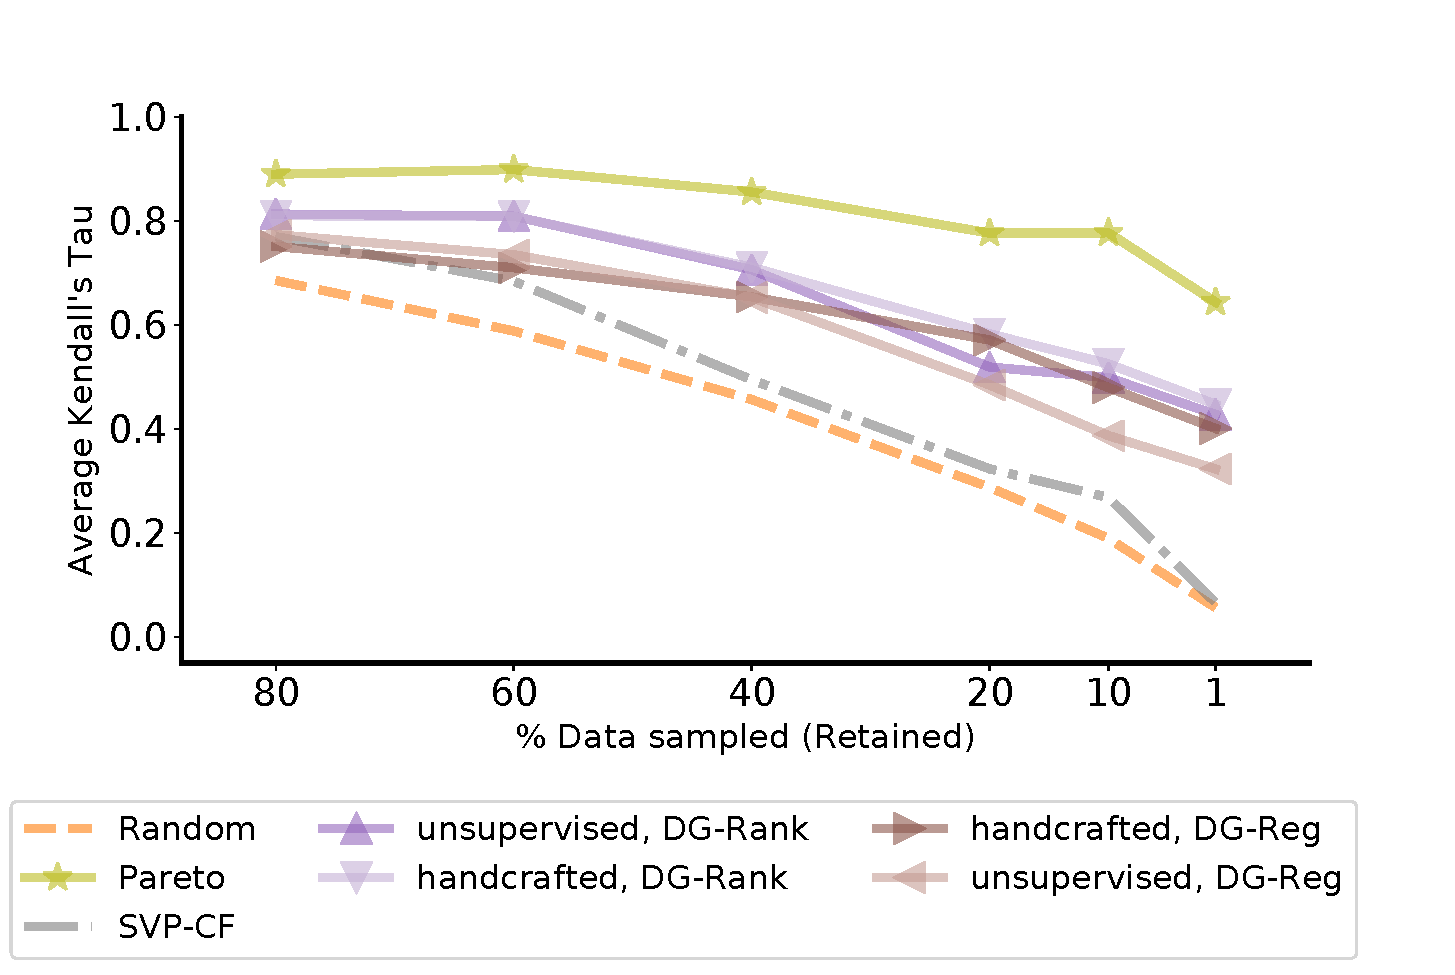
\includegraphics[width=0.86\linewidth]{figures/oracle_tau_vs_sampling_percent.pdf}
    \vspace{-0.1cm}
    \caption{Comparison of the average Kendall's Tau with \% data sampled for different sampling-selection strategies. A higher Tau indicates better retaining power of the ranking of different recommendation algorithms.}
    \label{percent_sampling_vs_tau_oracle}
\end{minipage}
\end{figure*} 

\subsection{Experiments}
\paragraph{Setup.} 
% We re-use the datasets, CF-scenarios, sampling strategies, and percentage sampling choices from \cref{main_exp}. To evaluate the competence of \oracle, we chose to perform the following train, validation, and test split: for each dataset and CF-scenario, we randomly split the metric and sampling percent $(m, p)$ join into $70/15/15\%$ proportions. Finally, during validation/testing, having fixed a dataset, CF-scenario, metric, and \% sampled data---we ask \oracle to predict the best sampler for this particular dataset. Given that there are only $16$ samplers in our study, we use the P$@1$ metric on the ranked list of samplers to evaluate \oracle.
We first create a train/validation/test split by randomly splitting all possible metrics and sampling $\%$ pairs $(m, p)$ into $70/15/15\%$ proportions. Subsequently for each dataset \dataset, CF-scenario $f$, and $(m, p)$ in the validation/test-set, we ask \oracle to rank all $16$ samplers (\cref{psi_results}) for $p\%$ sampling of $f-$type feedback for \dataset and use metric $m$ for evaluation by sorting $\hat{\tau}$ for each sampler, as defined in \cref{tau_hat}. To evaluate \oracle, we use the P$@1$ metric between the actual sampler ranking computed while computing $\Psi-$scores in \cref{main_exp}, and the one estimated by \oracle.
% Having already computed the true ranking of sampling strategies while computing $\Psi-$scores in \cref{main_exp}, we use the P$@1$ metric between the actual sampler ranking and the one estimated by sorting $\hat{\tau}$ for each sampler, as defined in \cref{tau_hat} to evaluate \oracle.

\subsubsection{How accurately can \oracle predict the best sampling scheme? \ \ } In \cref{oracle_results}, we compare all dataset representation choices $\mathcal{E}$, and multiple $\Phi$ architectures for the task of predicting the best sampling strategy. In addition to the regression and ranking architectures discussed in \cref{oracle_architecture}, we also compare with linear least-squares regression and XGBoost regression \cite{xgboost} as other choices of $\Phi$. In addition, we compare \oracle with simple baselines: (1) randomly choosing a sampling strategy; and (2) the best possible static sampler choosing strategy---always predict user sampling \emph{w/} Bias-only \samplerprop. First and foremost, irrespective of the $\mathcal{E}$ and $\Phi$ choices, \oracle outperforms both baselines. Next, both the handcrafted features and the unsupervised GCN features perform quite well in predicting the best sampling strategy, indicating that the graph characteristics are well correlated with the final performance of a sampling strategy. Finally, \oracle-regression and \oracle-ranking both perform better than alternative $\Phi-$choices, especially for the P$@1$ metric. 

% % \begin{table}[!ht]
    % \vspace{0.05cm}
    \begin{footnotesize} % normalsize, small, footnotesize
    \begin{center}
        \begin{tabular}{c c | c c c}
            \toprule
            $\mathcal{E}$ & $\Phi$ & \textbf{MSE} & \textbf{P@1} \\ \midrule
            
            \multicolumn{2}{c|}{Random} & 0.2336 & 25.2 \\ 
            \multicolumn{2}{c|}{User sampling \emph{w/} Bias-only \samplerprop} & -- & 30.6 \\ \midrule
            
            Handcrafted & Least squares regression & 0.1866 & 31.7 \\
            '' & XGBoost regression & 0.1163 & 43.9 \\
            '' & \oracle-regression & \underline{0.1008} & 51.2 \\ 
            '' & \oracle-ranking    & -- & 51.2 \\ \midrule
            
            Unsupervised GCN & Least squares regression & 0.1838 & 39.1 \\
            '' & XGBoost regression & 0.1231 & 43.9 \\
            '' & \oracle-regression & 0.1293 & 48.8 \\ 
            '' & \oracle-ranking    & -- & \underline{53.7} \\ \bottomrule
        \end{tabular}
    \end{center}
    \end{footnotesize}
    \vspace{0.5cm}
    \caption{Results for predicting the best sampling scheme for a particular dataset over a germane metric. The MSE-value next to randomly choosing the sampling scheme represents the variance of the test-set. Best values are \underline{underlined}.}
    \label{oracle_results}
    \vspace{-6mm} %Put here to reduce too much white space after your table
% \end{table}
% \begin{figure}[ht!] 
%     \centering
%     \vspace{-0.12cm}
%     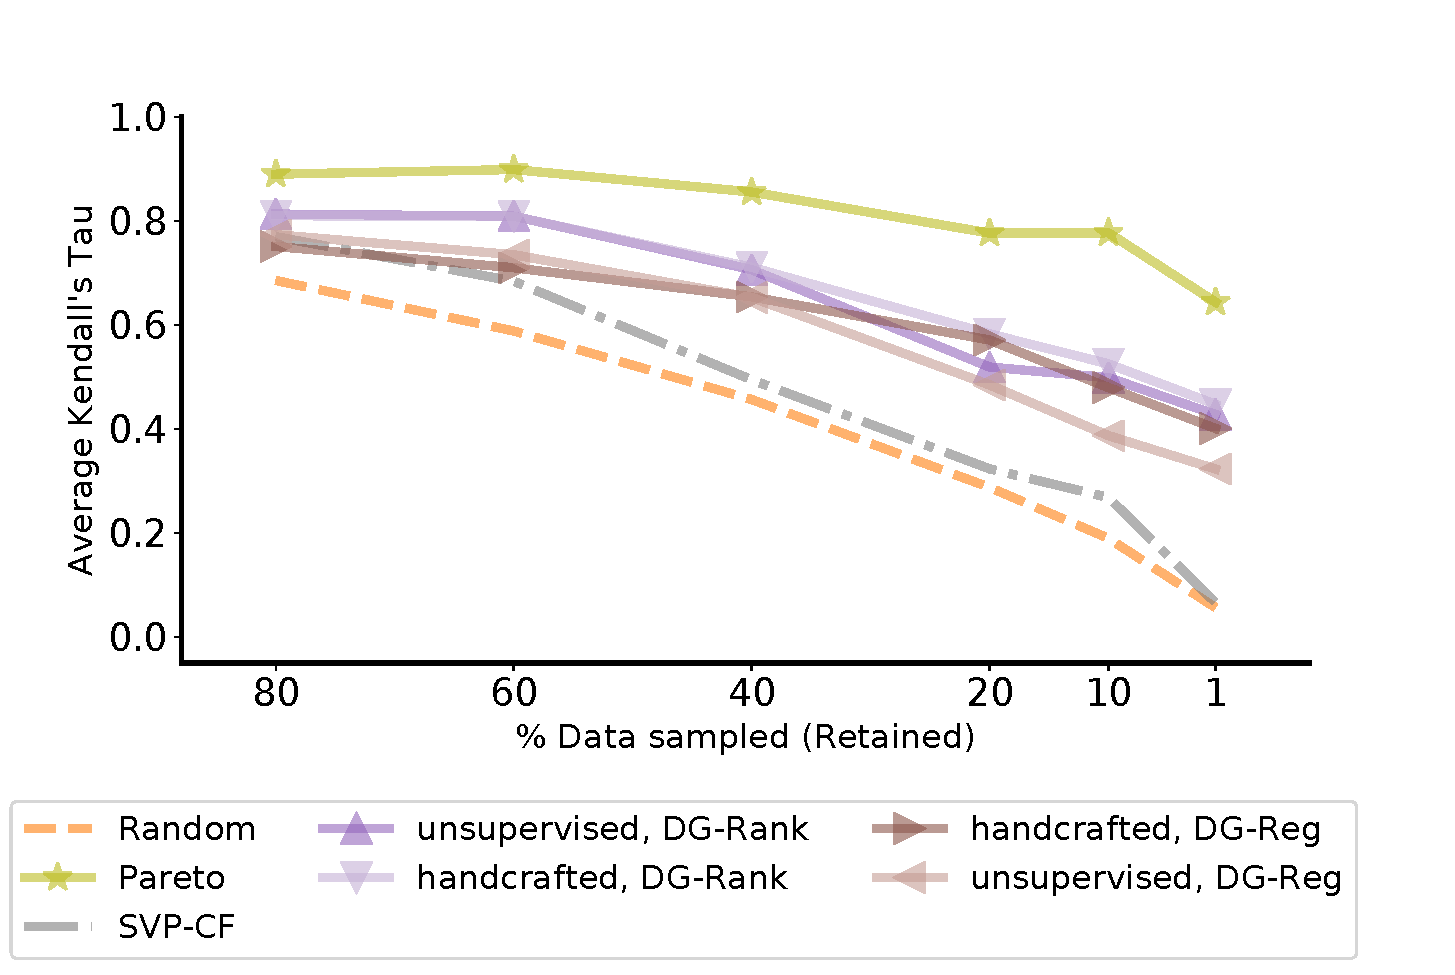
\includegraphics[width=\linewidth]{figures/oracle_tau_vs_sampling_percent.pdf}
%     \vspace{-0.5cm}
%     \caption{Comparison of the average Kendall's Tau with \% data sampled for different sampling-selection strategies. A higher Tau indicates better retaining power of the ranking of different recommendation algorithms.}
%     \label{percent_sampling_vs_tau_oracle}
% \end{figure} 

\subsubsection{Can we use \oracle to sample more data without compromising performance? \ \ } In \cref{percent_sampling_vs_tau_oracle}, we compare the impact of \oracle in sampling more data by dynamically choosing an appropriate sampler for a given dataset, metric, and $\%$ data to sample. 
% As a real-world benchmark for performance of \oracle, 
More specifically,
we compare the percentage of data sampled with the Kendall's Tau averaged over all datasets, CF-scenarios, and relevant metrics for different sampling strategy selection approaches. We compare \oracle with: (1) randomly picking a sampling strategy averaged over $100$ runs; and (2) the Pareto frontier as a skyline which always selects the best sampling strategy for any CF-dataset. As we observe from \cref{percent_sampling_vs_tau_oracle}, \oracle is better than predicting a sampling scheme at random, and 
% pushes the average Kendall's Tau
is
much closer to the Pareto frontier. Next, pairwise ranking approaches are marginally better than regression approaches 
% for both the handcrafted and unsupervised-GCN data features.
irrespective of $\mathcal{E}$. Finally, \oracle can appraise the best-performing recommendation algorithm with a suitable amount of confidence using only $10\%$ of the original data. This is significantly more efficient compared to having to sample $50-60\%$ if we were to always sample using a fixed strategy.